\section{実験・考察}\label{se4}

本章では,実施した利用評価実験の内容と結果および考察について述べる.

\subsection{利用評価実験}
本プラットフォームが,学習者に対し情報倫理に関するコンテンツを提供でき,そのコンテンツを見て学ぶことにより情報倫理に関するトラブルの減少とリテラシーの向上が期待できるかどうかを確認するために,利用評価実験を行った.
実験では20代男性10人に対して,本プラットフォームのコンテンツを事前に学習したコンテンツ利用者群と,事前に学習していないコンテンツ非利用者群の5人ずつに分かれて実験を行った.
そして各々の群に対し,GoogleFormを用いて全5問の情報倫理に関する問題を解いてもらった.
ただし,コンテンツ非利用者群に対してGoogleFormで問題を解くときに,わからない単語等があれば調べてもよいとした.

このような条件で実施したコンテンツ利用者群とコンテンツ非利用者群の実験結果を図\ref{result_all},図\ref{result_avg}に示す.
図\ref{result_all}はコンテンツ利用者群とコンテンツ非利用者群の獲得点数を表している.
図\ref{result_avg}はコンテンツ利用者群とコンテンツ非利用者群の獲得点数の平均と標準偏差を表している.

\begin{figure}[htbp]
    \begin{center}
        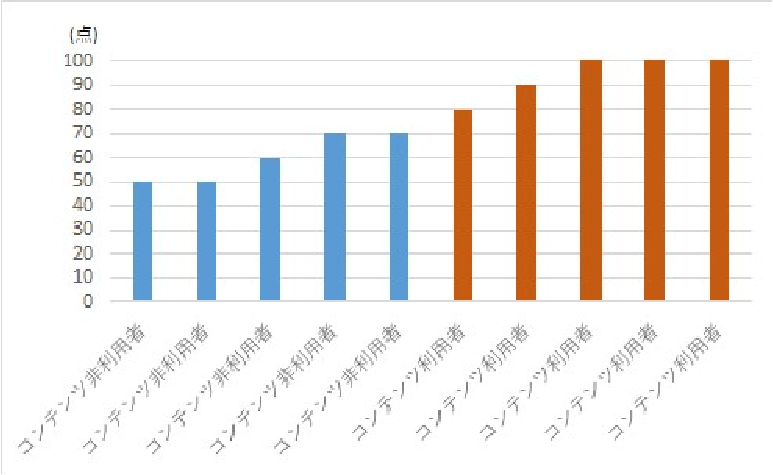
\includegraphics[width=13cm,height=12cm,keepaspectratio]{result_all-crop.pdf}\\
        %includegraphicsの詳しい使い方ははLaTeXの参考書を参照.
    \end{center}
    \caption{コンテンツ利用者群とコンテンツ非利用者群の獲得点数}
    \label{result_all}
\end{figure}
\newpage
\begin{figure}[htbp]
    \begin{center}
        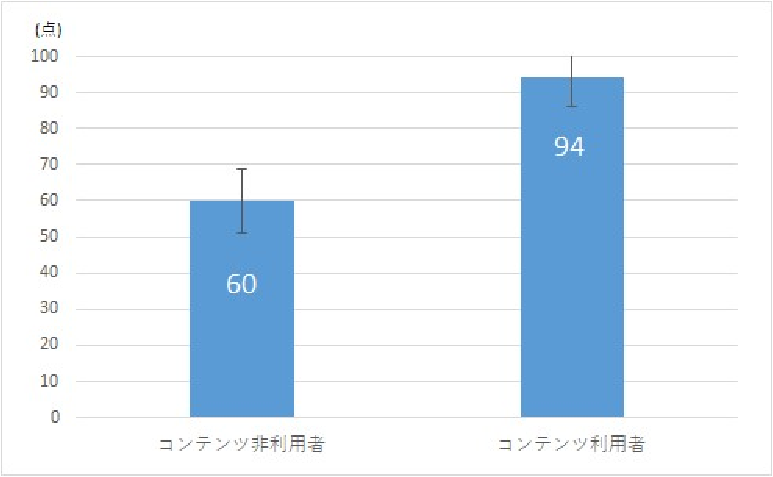
\includegraphics[width=13cm,height=12cm,keepaspectratio]{result-crop.pdf}\\
        %includegraphicsの詳しい使い方ははLaTeXの参考書を参照.
    \end{center}
    \caption{コンテンツ利用者群とコンテンツ非利用者群の獲得点数の平均と標準偏差}
    \label{result_avg}
\end{figure}

実験の結果,平均点においてコンテンツ利用者群が94点,コンテンツ非利用者群が60点と34点の差がついていることが分かった.
また,標準偏差においてはコンテンツ利用者群が 8.00,コンテンツ非利用者群が 8.94 であり,0.94 の差がついている.
以上から,本プラットフォームを用いて情報倫理について学習すると,点数のばらつきはコンテンツ利用者群の方がなく,点数も平均点の差からコンテンツ非利用者群と比べ高くなっていることがわかる.
このことからコンテンツ非利用者群は,情婦倫理に関して単語の記憶,理解だけを行っておりその結果情報倫理に対して十分な理解を得られずに問題を解き点数が低くなったと考えられる.
一方,コンテンツ利用者群は,本プラットフォームで提示したコンテンツを学んでいる.このコンテンツには実際に起こりうる情報倫理に関する問題をシナリオ形式で提示している.
このことによりコンテンツ利用者群は情報倫理に関して深く理解を得られたのではないかと考えられる.
したがって,本プラットフォームは学習者に対して,情報倫理に関するトラブルの減少とリテラシー向上を期待できる.
